\documentclass[fleqn]{article}
\oddsidemargin 0.0in
\textwidth 6.0in
\thispagestyle{empty}
\usepackage{import}
\usepackage{amsmath}
\usepackage{graphicx}
\usepackage{flexisym}
\usepackage{calligra}
\usepackage{amssymb}
\usepackage{bigints} 
\usepackage[english]{babel}
\usepackage[utf8x]{inputenc}
\usepackage{float}
\usepackage[colorinlistoftodos]{todonotes}


\DeclareMathAlphabet{\mathcalligra}{T1}{calligra}{m}{n}
\DeclareFontShape{T1}{calligra}{m}{n}{<->s*[2.2]callig15}{}
\newcommand{\scriptr}{\mathcalligra{r}\,}
\newcommand{\boldscriptr}{\pmb{\mathcalligra{r}}\,}

\definecolor{hwColor}{HTML}{442020}

\begin{document}

  \begin{titlepage}

    \newcommand{\HRule}{\rule{\linewidth}{0.5mm}}

    \center

    \begin{center}
      
\includegraphics[height=11cm, width=11cm]{asu.png}
    \end{center}

    \vline

    \textsc{\LARGE Statistical/Thermal Physics}\\[1.5cm]

    \HRule \\[0.5cm]
    { \huge \bfseries Quiz 9}\\[0.4cm] 
    \HRule \\[1.0cm]

    \textbf{Behnam Amiri}

    \bigbreak

    \textbf{Prof: Michael Treacy}

    \bigbreak

    \textbf{{\large \today}\\[2cm]}

    \vfill

  \end{titlepage}

  By signing my name, I am promising that I did this quiz on my own without any outside help.

  \vspace{0.5cm}

  Name: \textbf{Behnam Amiri}

  \vspace{1cm}

  \begin{center}
    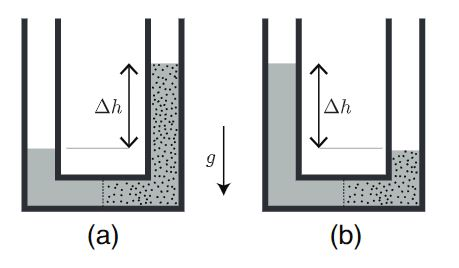
\includegraphics[height=5cm, width=10cm]{1.JPG}
  \end{center}

  The figure shows two possible experimental arrangements to measure the osmotic pressure across
  a membrane (which is represented by the vertical dashed line at the bottom of (a) and (b)). Gravity
  acts downwards. In each figure, the pure solvent (i.e. pure A) is on the left of the membrane, and
  the solution (i.e. A with some B solute dissolved in it) is on the right of the membrane. The
  membrane is semi-permeable, meaning that solvent A molecules can diffuse through it, but not
  solute B molecules.

  \begin{enumerate}
    \item \textbf{(10 points)} Which one of the following statements is true?
      \begin{enumerate}
        \item Osmotic flow through the membrane is undisturbed by the difference in fluid levels.

          \textcolor{hwColor}{
            \\
            For an osmotic flow this is wrong.
            \\
          }


        \item In setup (a), solute molecules from the right are being “pushed” by the hydrostatic pressure
        difference through the membrane into the pure solvent on the left.

          \textcolor{hwColor}{
            \\
            This is wrong.
            \\
          }

        \item In setup (b), solvent molecules from the right are being “sucked” through the membrane
        into the pure solvent on the left, concentrating the solution on the right, and creating a
        hydrostatic pressure difference.

          \textcolor{hwColor}{
            \\
            No, this statement is wrong.
            \\
          }

        \item  In setup (a), the net flow of solvent molecules through the membrane, from the left to
        the right, can be stopped or reversed if the hydrostatic pressure difference, caused by the
        difference in fluid heights $\Delta h$, is sufficiently large.

          \textcolor{hwColor}{
            \\
            Yes, this statement is correct.
            \\
          }

        \item In setup (b), solvent molecules are spontaneously flowing out of the solution on the right
        and are being collected in pure form on the left, causing the difference in heights, ∆h. This
        is the principle of \emph{reverse osmosis}.

          \textcolor{hwColor}{
            \\
            No, this statement is wrong.
            \\
          }

      \end{enumerate}

    \item \textbf{(10 points)} Hemoglobin is a large protein molecule that can be dissolved in water in dilute
    concentrations. In setup (a) (see Figure), the hemoglobin solution is on the right, with con-
    centration 16.6 grams/liter, and pure water is on the left. The semi-permeable membrane will
    let water through, but not hemoglobin. Hemoglobin solution is added to the right side until
    the pressure difference caused by the $\Delta h$ is sufficient to stop the net flow of water through the
    membrane. This is found to occur at $\Delta h = 6.5$ cm when the temperature is $3^{\circ} C$.
    Use the van't Hoff's formula (5.78) to estimate the molecular weight of hemoglobin. (Hint:
    $\Delta P= \rho g \Delta h$, where $\rho$ is the solution density.)

      \textcolor{hwColor}{
        \\
        On page 204 of the textbook we learned about the \textbf{Van't Hoff's} equation.
        \\
        \\
        $
          \Delta P=P_2-P_1=\dfrac{nRT}{V}
          \\
          \\
          \begin{cases}
            R=8.314 ~ J/mol.K
            \\
            \\
            T=3^{\circ} C+273.15=276.15 ~ K
            \\
            \\
            \rho=997 ~ kg/m^3
          \end{cases}
          \\
          \\
          \\
          \Delta P= \rho g \Delta h
          =\bigg( 997 ~ kg/m^3 \bigg) \bigg( 9.807 ~ m/s^2 \bigg) \bigg( 6.5 \times 10^{-2} ~ m \bigg)
          =635.54 ~ Pa=0.006272 ~ atm
          \\
          \\
          \\
          \text{Mass}=\dfrac{16.6 \times RT}{\Delta P ~ V}
          =\dfrac{16.6 \times 8.314 \times 10^{-2} \times 276.15}{0.006272}
          \\
          \\
          \\
          \therefore ~~~ \boxed{
            \text{Mass}=60765.5 ~ \text{grams}
          } ~~~~ \checkmark
          \\
          \\
        $
      }

    \item \textbf{(10 points)} Consider a large system of hypothetical atoms that have just two energy states: a
    ground state with zero energy, and an excited state at $0.01 ~ eV$. Estimate the mean energy per
    atom at $T=300 ~ K$.

      \textcolor{hwColor}{
        \\
      }

  \end{enumerate}

\end{document}
